\documentclass[a4paper,twocolumn]{article}

\usepackage{graphicx}          % To handle figures
\usepackage{amsmath}           % Defines certain mathematical symbols
%\usepackage{psfrag}            % Inserts LaTeX text into figures (does not work with PDFLatex)
\usepackage{url}               % To typeset email addresses and URLs
\usepackage[latin1]{inputenc}  % Makes sure that all Swedish characters
                               % work
%\usepackage[swedish]{babel}    % If you want to write in Swedish.

\addtolength{\topmargin}{-25mm}% Decrease the top margin by 25mm
\addtolength{\textheight}{25mm}% Increase the text height by the
                               % same amount

\begin{document}

\title{An Appropriate Title for the Report}
\author{Firstname1 Familyname1 \\ Personalnumber1 \and Firstname2 Familyname2\\
  Personalnumber2}
%\date{2000-10-10} % If you don't want todays date.

\maketitle


\begin{abstract}
  The summary/abstract is perhaps the most important part of a
  report. Here you should catch the attention of the reader. Bring up
  the problem you want to solve and briefly summarize your results.
\end{abstract}

\section{Introduction}
\label{sec:intro}

Always include a brief introduction to the problems. Specify at an
early stage what problem you intend to solve, i.e. define the
problem. It is a good idea to bring up different practical
applications.

Introduce the data models that are used and describe clearly all the
necessary assumptions. This is crucial, since otherwise the reader
will probably not be able to follow the rest of the report.

\section{Theory}
\label{sec:theory}

Often you need to present some theoretical results.

If you include equations, it is convenient to be able to reference
them by number, as in Equation~\eqref{eq:datamodel}.
\begin{equation}
  \label{eq:datamodel}
  y(t) = h(t) \ast x(t)
\end{equation}

\section{Numerical Results}
\label{sec:numerical}

It is common to include numerical examples to illustrate the
theoretical results (from Section~\ref{sec:theory}).

\begin{figure}[!ht]
  \begin{center}
    % Standard LaTeX can handle EPS files.
    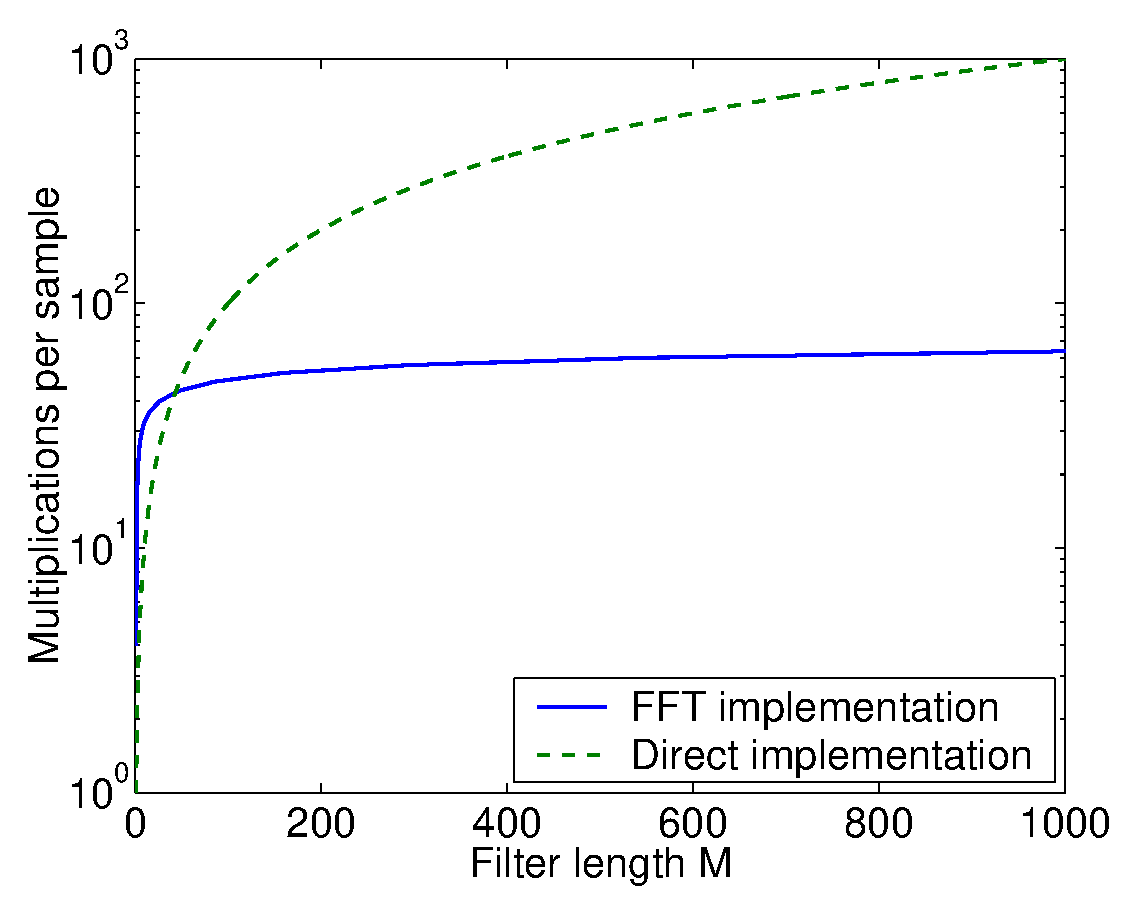
\includegraphics[width=0.83\columnwidth]{optComp.eps}
    % If you instead use pdflatex to process the file, the
    % figures should be in PDF, JPG or PNG format.
  \end{center}
  \caption{Always specify the unit of the axes.}
  \label{fig:performance}
\end{figure}
A figure is often more informative than text or tables, but make sure
to only include relevant figures and to describe and reference them
from the text, see for example Figure~\ref{fig:performance}.


\section{Conclusions}
\label{sec:conclusions}

Summarize and draw some sensible conclusions. Some hints:
\begin{itemize}
\item Do not just list questions from the project instructions with
  the corresponding answers. Instead, try to include the results in
  running text.
\item Preferably, it should be possible to reproduce your results
  based on the information in the report, without having access to the
  project instructions.
\end{itemize}

\section*{Appendix}

In an appendix, you could add details that are not necessary to follow
the main ideas of the report, but still could be of interest to some
readers, such as detailed proofs. Do not include MATLAB code, though.

This report is typeset using \LaTeXe. A good introduction to \LaTeXe
is available in \cite{latexmanual}. Feel free to use any other word
processor if you prefer.

%The pictures used in the project descriptions are included as follows (and takes up a double column spacing). This however requires the psfrag package which does not work together with PDF LaTeX
%
%\begin{figure*}[htbp]
%  \begin{center}
%    \psfrag{H0}[][]{$H_0(z)$}
%    \psfrag{H1}[][]{$H_1(z)$}
%    \psfrag{y}[][]{$y(n)$}
%    \psfrag{y1}[][]{$y_1(n)$}
%    \psfrag{y01}[][]{$y_{01}(n)$}
%    \psfrag{y00}[][]{$y_{00}(n)$}
%    \psfrag{z1}[l][l]{$z_1(n)$}
%    \psfrag{z01}[l][l]{$z_{01}(n)$}
%    \psfrag{z00}[l][l]{$z_{00}(n)$}
%    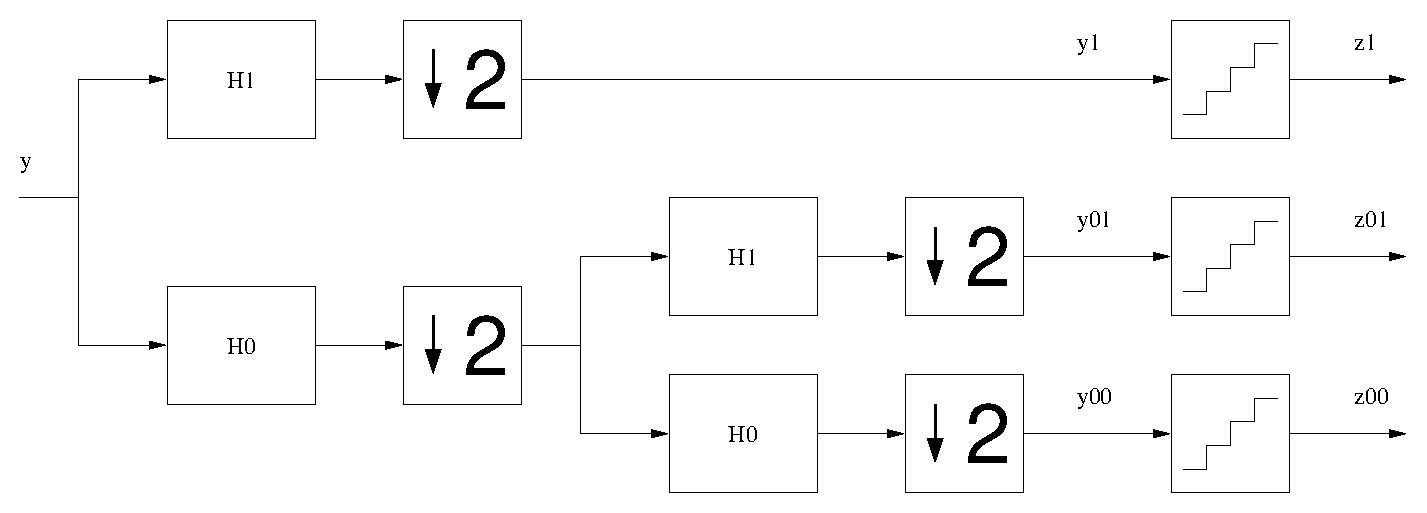
\includegraphics[height=4cm]{analysisbank3}
%    \caption{Analysis filter bank followed by quantization.}
%    \label{fig:analysisbank3}
%    \bigskip\bigskip
%    \psfrag{G0}[][]{$G_0(z)$}
%    \psfrag{G1}[][]{$G_1(z)$}
%    \psfrag{v}[][]{$v(n)$}
%    \psfrag{zl}[][]{$z^{-l}$}
%    \psfrag{z1}[r][r]{$z_1(n)$}
%    \psfrag{z01}[r][r]{$z_{01}(n)$}
%    \psfrag{z00}[r][r]{$z_{00}(n)$}
%    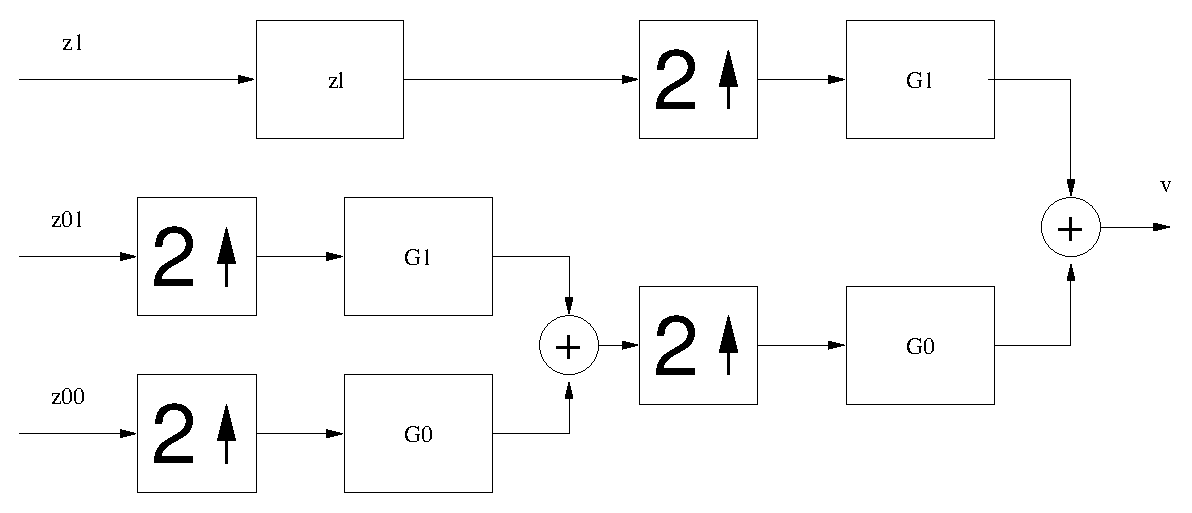
\includegraphics[height=4cm]{synthesisbank3}
%    \caption{Synthesis filter bank.}
%    \label{fig:synthesisbank3}
%  \end{center}
%\end{figure*}

\begin{thebibliography}{99}
\bibitem{latexmanual} Tobias Oetiker et al. \textsl{The Not So Short
    Introduction to
    \LaTeXe}
    \url{www.tex.ac.uk/tex-archive/info/lshort/english/lshort.pdf}.
\end{thebibliography}
\end{document}
